
% !TeX spellcheck = en_US

\documentclass{beamer}

\usepackage{authblk,fullpage,amsfonts,amssymb,theorem}
\usepackage{graphicx,hyperref}
\usepackage{ragged2e}
\usepackage{tikz}
\usepackage{booktabs}
\usepackage{bm}

\usepackage{tikz}
\usetikzlibrary{shapes,arrows, positioning}

\tikzset{
	treenode/.style = {shape=rectangle, rounded corners,
		draw, align=center, text width=10em,
		fill=red!15},
	root/.style     = {diamond, draw, fill=blue!20,
		text width=6em, text badly centered, node distance=3cm, inner sep=0pt},
	env/.style      = {treenode, font=\ttfamily\normalsize},
	dummy/.style    = {circle,draw},
	curve/.style={->, thick, >=stealth'},
}
\tikzstyle{line} = [draw, -latex']
\tikzstyle{bag} = [text width=3em, text centered]
\tikzstyle{end} = [rectangle, draw=none, minimum width=2pt, inner sep=0pt]


\mode<presentation> {

% The Beamer class comes with a number of default slide themes
% which change the colors and layouts of slides. Below this is a list
% of all the themes, uncomment each in turn to see what they look like.

%\usetheme{default}
%\usetheme{AnnArbor}
%\usetheme{Antibes}
%\usetheme{Bergen}
%\usetheme{Berkeley}
%\usetheme{Berlin}
%\usetheme{Boadilla}
%\usetheme{CambridgeUS}
%\usetheme{Copenhagen}
%\usetheme{Darmstadt}
%\usetheme{Dresden}
%\usetheme{Frankfurt}
%\usetheme{Goettingen}
%\usetheme{Hannover}
%\usetheme{Ilmenau}
%\usetheme{JuanLesPins}
%\usetheme{Luebeck}
\usetheme{Madrid}
%\usetheme{Malmoe}
%\usetheme{Marburg}
%\usetheme{Montpellier}
%\usetheme{PaloAlto}
%\usetheme{Pittsburgh}
%\usetheme{Rochester}
%\usetheme{Singapore}
%\usetheme{Szeged}
%\usetheme{Warsaw}

% As well as themes, the Beamer class has a number of color themes
% for any slide theme. Uncomment each of these in turn to see how it
% changes the colors of your current slide theme.

%\usecolortheme{albatross}
\usecolortheme{beaver}
%\usecolortheme{beetle}
%\usecolortheme{crane}
%\usecolortheme{dolphin}
%\usecolortheme{dove}
%\usecolortheme{fly}
%\usecolortheme{lily}
%\usecolortheme{orchid}
%\usecolortheme{rose}
%\usecolortheme{seagull}
%\usecolortheme{seahorse}
%\usecolortheme{whale}
%\usecolortheme{wolverine}

%\setbeamertemplate{footline} % To remove the footer line in all slides uncomment this line
\setbeamertemplate{footline}[page number] % To replace the footer line in all slides with a simple slide count uncomment this line

\setbeamertemplate{navigation symbols}{} % To remove the navigation symbols from the bottom of all slides uncomment this line
}

\usepackage{graphicx} % Allows including images
\usepackage{booktabs} % Allows the use of \toprule, \midrule and \bottomrule in tables
%\usepackage {tikz}

\setbeamertemplate{caption}[numbered]

\AtBeginSection[]{
	\begin{frame}
		\vfill
		\centering
		\begin{beamercolorbox}[sep=8pt,center,shadow=true,rounded=true]{title}
			\usebeamerfont{title}\insertsectionhead\par%
		\end{beamercolorbox}
		\vfill
	\end{frame}
}

%\usepackage {xcolor}
\definecolor {processblue}{cmyk}{0.96,0,0,0}
%----------------------------------------------------------------------------------------
%	TITLE PAGE
%----------------------------------------------------------------------------------------

\title[Short title]{Momentum Gender Gap} % The short title appears at the bottom of every slide, the full title is only on the title page

\author{Sofiya Malamud \and Jiahua (Java) Xu} % Your name
\institute[EPFL]
{
	Sofiya Malamud \and Jiahua (Java) Xu
%Swissquote, EPFL,UCL \\ % Your institution for the title page
\medskip
}
\date{\today} % Date, can be changed to a custom date

\begin{document}

\begin{frame}
\titlepage % Print the title page as the first slide
\end{frame}

%\begin{frame}
%\frametitle{Overview} % Table of contents slide, comment this block out to remove it
%\tableofcontents % Throughout your presentation, if you choose to use \section{} and \subsection{} commands, these will automatically be printed on this slide as an overview of your presentation
%\end{frame}

%----------------------------------------------
%	PRESENTATION SLIDES
%----------------------------------------------


\begin{frame}{Key findings}

\begin{enumerate}[A]
	\item Female Traders have a preference for Momentum stock
	\item Women are more prone towards the disposition effect
	\item Female trading has a higher correlation towards future asset performance than general momentum trading 
	\item Women are able to generate higher returns than their male counterparts
\end{enumerate}

\end{frame}



\section{Research motivation and background}


\begin{frame}{Purpose of the study}


Study the impact of female momentum trading on future asset performance

%	\begin{enumerate}
%		\item{Trading platforms}
%		\begin{itemize}
%			\item should focus on retaining inexperienced traders
%		\end{itemize}
%
%		\item{Investors}
%		\begin{itemize}
%			\item should understand their trading inertia might not be economically rational
%		\end{itemize}
%	\end{enumerate}


\end{frame}


\begin{frame}{Literature review}

	\begin{itemize}
	    \item \cite{Shefrin1985}: Hypothesize female traders are more prone towards the disposition effect
		\item \cite{Lu2017}: Show that female traders outperform their male counterparts
		\item \cite{JEGADEESH1993}: Show that past winning stocks over the last 6 months continue outperforming past losing stocks

		%		Also relevant for our study is the literature on the trading behavior of different investor cohorts.  \cite{Grinblatt2001} show that domestic and less sophisticated investors tend to be reversal traders, whereas foreign and more sophisticated investors tend to be trend followers. \cite{Dorn2005} investigate the relationship between investor behaviors and objective attributes such age, gender and income, as well as subjective attributes such as self-reported risk attitude. They find that investors with high risk tolerance and who believe themselves to be more knowledgeable than the average trade more aggressively. \cite{Kourtidis2011} find that wealthy and educated individuals are associated with higher risk tolerance and more frequent trading.
		%
		%		Our research is also informed by the vast literature on investor psychology. Many such research studies focus on investor overconfidence demonstrated by excessive and/or aggressive trading. \cite{Odean1998} proves that overconfidence in one's information increases one's trading volume, and that overconfidence when manifested by miscalibration, decreases the expected utility of overconfident traders. \cite{Odean1999} demonstrates that investors with reduced trading costs tend to trade excessively, resulting in unsuccessful investments. \cite{Glaser2007} find that investors' overconfidence, when measured by better-than-average effect, is positively related to trading volume; overconfidence measured by miscalibration, however, has little to do with trading volume. \cite{Barber2000} conclude that individuals who trade excessively often gain lower net returns as the superior trading performance does not always compensate for the higher trading costs. \cite{Daniel2015} suggest that unprofitable but excessive active trading can be explained by overconfident beliefs in one's own talents and abilities.
		%
		%		Other research studies discuss the disposition effect --  to sell winners and ride losers – a theory established by  \cite{Shefrin1985}. \cite{Odean1998a} demonstrates investors preference for realizing winners over losers, except in the tax optimizing period of December. \cite{Dhar2006} suggest educated individuals exhibit lower disposition bias than their less literate peers. Relatedly, \cite{Kahneman1979} suggest people unwilling to accept losses tend to engage in gambles that are riskier than they would normally tolerate.

	\end{itemize}

\end{frame}


\section{Data and Methodology}

\begin{frame}{Sample collection}

\begin{itemize}
	\item Source: one of the biggest stock trading platforms for retail traders in Switzerland
 \item Number of clients : 89,662

\item Number of trades :  2,314,257

\item Average number of trades per client per month : 10.7

\item Gender composition : 12,038 women and 77,624 men 

\item Average number of trades per month : 7,541 

\end{itemize}

\end{frame}


\begin{frame}{Hypothesises we test}

\begin{itemize}

	\item Do women favor momentum stock ?

	\item Are women prone towards the disposition effect?
	
	\item How does female momentum Trading affect future asset performance?
	
	\item Do female traders come out on top compared to male traders?

\end{itemize}
\end{frame}


%\begin{frame}{Initial belief distribution}
%	Inverse exponential distribution on
%	$[\ell - \ell_*(0, \varphi), +\infty)$
%
%	\begin{columns}[t]
%		\begin{column}{0.49\textwidth}
%			\begin{block}{$\varphi = 0.01$}
%				\begin{figure}
%					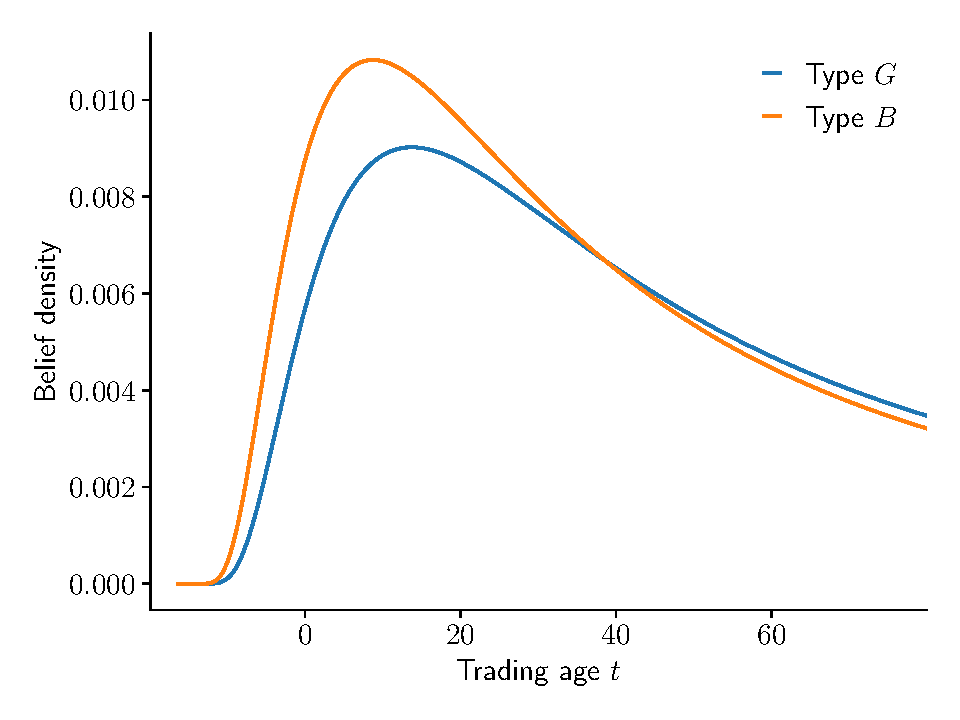
\includegraphics[width=\linewidth]{figures/ldist1}
%				\end{figure}
%			\end{block}
%		\end{column}
%
%		\begin{column}{0.49\textwidth}
%			\begin{block}{$\varphi = 9$}
%				\begin{figure}
%					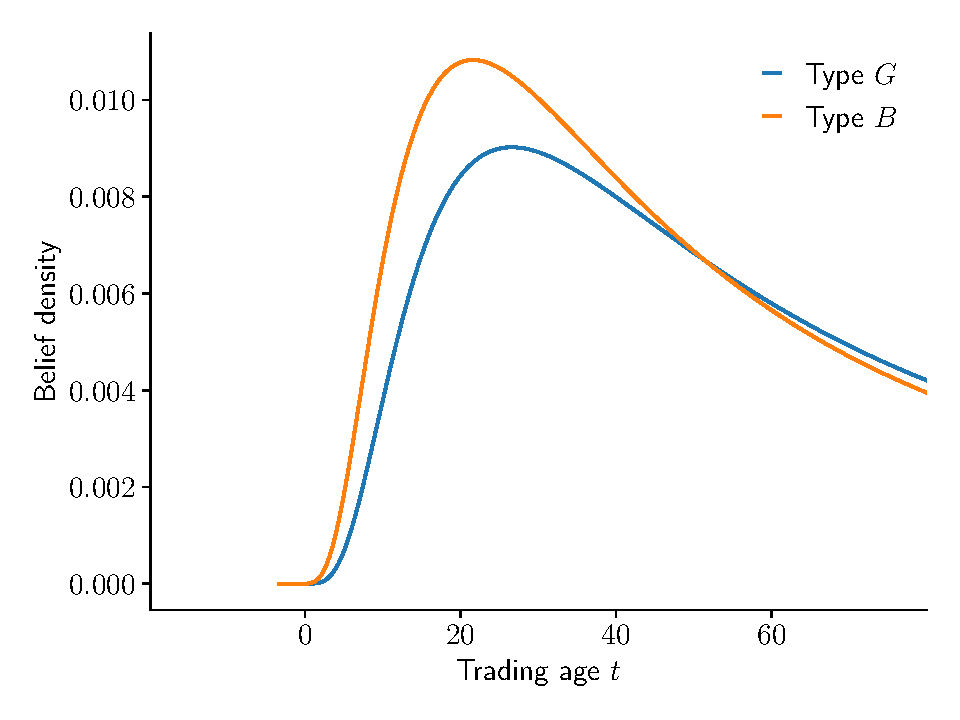
\includegraphics[width=\linewidth]{figures/ldist2}
%				\end{figure}
%			\end{block}
%		\end{column}
%	\end{columns}
%\end{frame}


\section{Empirical results}

\begin{frame}{Women favor Momentum Stock and are prone towards the disposition effect}
\begin{equation}
    \label{eq:womanbuysell} 
    \tiny
    {\bf 1}_{women, t}(i) = \sum_{k=1}^K\beta_k^{w,b} X_{k,t}(i)\ +\ \epsilon_t^{w,s}(i)
\end{equation}
\begin{table}[htbp]
    \centering
    \caption{Effects of momentum on female buy and sell decisions }
    \label{tab:regression1}
    \tiny
\begin{tabular}{ lrrrr } 
 \multicolumn{1}{c}{} \\
 \toprule
  Regressions & \eqref{eq:womanbuysell} with buys & \eqref{eq:womanbuysell} with sells  \\ 
   \midrule 
 Intercept   &\shortstack{$-1.887$*** \\ (660)} & \shortstack{$-0.594$*** \\ (324)}  \\ 
  
 ret-measure-250 & \shortstack{0.125*** \\ (26.50)} & \shortstack{$-0.017$*** \\ (5.209)} \\ 
 
 ret-measure-70& \shortstack{0.021* \\ (2.089) }& \shortstack{ 0.022**  \\ (3.100)}\\
 
 ret-measure-25 & \shortstack{$-0.065$*** \\ (4.973)} & \shortstack{$-0.081$*** \\ (9.051)}  \\
 
 $|$ret-measure-250$|$ & \shortstack{$-0.180$*** \\ (11.37)} &  \shortstack{0.117*** \\ (1)}  \\ 
 
 $|$ret-measure-70$|$ & \shortstack{$-0.094$*** \\ (7.631)}  &  \shortstack{0.030***  \\ (3.550)} \\ 
 
 $|$ret-measure-25$|$ & \shortstack{$-0.100$*** \\ (16.11)}  &  \shortstack{$-0.074$***  \\ (16.69)} \\ 
 \bottomrule
\end{tabular}

\end{table}

\end{frame}

\begin{frame}{Female and Male "attractiveness" measures towards certain stocks}

\begin{itemize}
\item First : attractiveness of a stock in a given month among women
\item Second: captures its attractiveness among all clients too women . 
\begin{equation}
\begin{aligned}
    & FB^1_{i,t}\ =\ \frac{\#\ women\ who\ bought\ stock\ in\ month\ t}{\#\ women\ who\ bought\ some\ stock\ in\ month\ t}\\
    & FB^2_{i,t}\ =\ \frac{\#\ women\ who\ bought\ stock\ in\ month\ t}{\#\ clients\ who\ bought\ this\ particular\ stock\ in\ month\ t}
\end{aligned}
\end{equation}
\item First : attractiveness of a stock in a given month among men
\item Second: captures its attractiveness among all clients too men. 
\begin{equation}
\begin{aligned}
    & MB^1_{i,t}\ =\ \frac{\#\ men\ who\ bought\ stock\ in\ month\ t}{\#\ men\ who\ bought\ some\ stock\ in\ month\ t}\\
    & MB^2_{i,t}\ =\ \frac{\#\ men\ who\ bought\ stock\ in\ month\ t}{\#\ clients\ who\ bought\ this\ particular\ stock\ in\ month\ t}
\end{aligned}
\end{equation}
\item Same measures are constructed but using data on sales

\end{itemize}

\end{frame}

\begin{frame}{Testing for correlation between asset performance and female and male buy trades}

\begin{equation}
\label{eq:FB}
     R_{t,t+25}(i) = \alpha + \sum_{k=1}^K\beta_k X_{k,t}(i)\ +\ \beta^{FB} FB_{i,t}\ + \sum_{k=1}^K\beta_k^{w,b} X_{k,t}(i)FB_{i,t}  + \epsilon_{t+1}
\end{equation}
\begin{equation}
\label{eq:MB}
     R_{t,t+25}(i) = \alpha + \sum_{k=1}^K\beta_k X_{k,t}(i)\ +\ \beta^{MB} MB_{i,t}\ + \sum_{k=1}^K\beta_k^{w,b} X_{k,t}(i)MB_{i,t}  + \epsilon_{t+1}
\end{equation}

\end{frame}

\begin{frame}{Future asset performance correlation towards female and male buy Trades}

\begin{table}[htbp]
    \centering
    \caption{Regression results using female and male buy attractiveness scores}
    \label{tab:FB-MB}
     \tiny
\begin{tabular}{ lrrrr } 
 \multicolumn{1}{c}{} \\
 \toprule
 Regressors & $FB^1_{i,t}$ & $FB^2_{i,t}$ & $MB^1_{i,t}$ & $MB^2_{i,t}$  \\ 
  \midrule
Intercept  & \shortstack{$-0.011$*** \\ (83.71)} & \shortstack{$-0.011$*** \\ 68.52)} & \shortstack{$-0.009$*** \\ (74.24)} &  \shortstack{0.008*** \\ (9.425)}\\

ret-measure-25  & \shortstack{$-0.059$*** \\ (74.92)}& \shortstack{$-0.0753$*** \\ (79.92)} & \shortstack{$-0.053$*** \\ (67.64)} &  \shortstack{0.001 \\ 0.197)}\\

ret-measure-70  & \shortstack{$-0.033$*** \\ (4.723)} & \shortstack{0.010*** \\ (13.79)} & \shortstack{$-0.0007$ \\ (1.21)} & \shortstack{0.046*** \\ (10.79)} \\

ret-measure-250 & \shortstack{ 0.019*** \\ (67.74)}& \shortstack{0.015*** \\ (44.82)} & \shortstack{0.019*** \\ (67.98)} & \shortstack{$-0.014$*** \\ (7.841)}\\

indicator & \shortstack{0.188*** \\ (31.08)}& \shortstack{0.019*** \\ (19.80)} &\shortstack{0.025*** \\ (6.399)} & \shortstack{$-0.019$*** \\ (19.80)}\\

indicator:ret-measure-25 & \shortstack{ $-0.691$*** \\ (17.39)}& \shortstack{ 0.076*** \\ (11.90)} & \shortstack{$-0.718$*** \\ (31.48)} & \shortstack{$-0.076$*** \\ (11.90)}\\

indicator:ret-measure-70 & \shortstack{2.049*** \\ (60.25)}& \shortstack{0.036*** \\ (7.609)} & \shortstack{1.021*** \\ (53.52)} & \shortstack{$-0.036$*** \\ (7.609)}\\

indicator:ret-measure-250 & \shortstack{$-0.965$ \\ (53.04)}***& \shortstack{$-0.029$*** \\ (14.26)} & \shortstack{ $-0.522$*** \\ (52.21)} & \shortstack{0.029*** \\ (14.26)}\\

\cr

Multiple $R^2$ &0.007& 0.059 & 0.007 & 0.005\\

Adjusted $R^2$ &0.007&0.005 & 0.007 & 0.006\\
 \bottomrule
\end{tabular}

\end{table}

\begin{frame}{Testing for correlation between asset performance and female and male sell trades}

\begin{equation}
\label{eq:FS}
     R_{t,t+25}(i) = \alpha + \sum_{k=1}^K\beta_k X_{k,t}(i)\ +\ \beta^{FS} FS_{i,t}\ + \sum_{k=1}^K\beta_k^{w,b} X_{k,t}(i)FS_{i,t}  + \epsilon_{t+1}
\end{equation}

\begin{equation}
\label{eq:MS}
     R_{t,t+25}(i) = \alpha + \sum_{k=1}^K\beta_k X_{k,t}(i)\ +\ \beta^{MS} MS_{i,t}\ + \sum_{k=1}^K\beta_k^{w,b} X_{k,t}(i)MS_{i,t}  + \epsilon_{t+1}
\end{equation}

\end{frame}

\begin{frame}{Future asset performance correlation towards female and males sell Trades}

\begin{table}[htbp]
    \centering
    \caption{Regression results using $FS^1_{i,t}$, $FS^2_{i,t}$, $MS^1_{i,t}$, $MS^2_{i,t}$}
    \label{tab:FS-MS}
    \tiny
\begin{tabular}{ lrrrr } 
 \multicolumn{1}{c}{} \\
 \toprule
 Regressors & $FS^1_{i,t}$ & $FS^2_{i,t}$ & $MS^1_{i,t}$ & $MS^2_{i,t}$  \\ 
  \midrule
Intercept  & \shortstack{0.007*** \\ (67.78)}& \shortstack{$-0.011$*** \\ (41.60)} & \shortstack{$-0.009$*** \\ (75.47)} &  \shortstack{0.005*** \\ (14.35)}\\

ret-measure-25  & \shortstack{$-0.083$*** \\ (127)}&  \shortstack{$-0.109$*** \\ (82.89)} & \shortstack{$-0.067$*** \\ (98.35)} &  \shortstack{0.005*** \\ (18.98)}\\

ret-measure-70  & \shortstack{ $-0.011$*** \\ (19.98)} & \shortstack{ $-0.0004$ \\  (0.435)}& \shortstack{ 0.008***  \\ (14.71)}& \shortstack{0.068*** \\ (37.80)} \\

ret-measure-250 & \shortstack{0.025*** \\ (104)}& \shortstack{0.022*** \\ (45.55)} & \shortstack{0.029*** \\ (112)} & \shortstack{$-0.008$*** \\ (10.35)}\\

indicator & \shortstack{0.035*** \\ (34.09)}& \shortstack{0.016*** \\ (25.62)} &\shortstack{0.098*** \\ (48.21)} &  \shortstack{$-0.016$*** \\ (25.63)}\\

indicator:ret-measure-25 & \shortstack{0.077*** \\ (8.934)}& \shortstack{0.069*** \\ (21.42)} & \shortstack{$-0.484$*** \\ (28.61)} & \shortstack{$-0.069$*** \\ (21.43)}\\

indicator:ret-measure-70 & \shortstack{0.244*** \\ (36.20)}& \shortstack{0.068*** \\ (24.51)} & \shortstack{0.468*** \\ (35.27)} & \shortstack{$-0.068$*** \\ (24.52)}\\

indicator:ret-measure-250 & \shortstack{$-0.278$*** \\ (90.91)}& \shortstack{0.031*** \\ (24.70)} & \shortstack{0.595***  \\ (98.78)}& \shortstack{0.031*** \\ (24.71)}\\

\cr

Multiple $R^2$ &0.011& 0.009& 0.012 & 0.009\\

Adjusted $R^2$ &0.011&0.009 & 0.012& 0.009\\
 \bottomrule
\end{tabular}
\end{table}

\end{frame}

\begin{frame}{Synthetic dollar neutral portfolio}
\begin{itemize}
    \item Using a signal $S_{i,t}$ that positively predicts returns we build a dollar-neutral portfolio by taking a long position in stocks with a large $S_{i,t}$, and a short position in stocks with a low $S_{i,t}.$ 
    \item The most common way of doing this (following \cite{Fama1993}) is to sort signals, $S_{i,t},$ pick their  $20\%$ and $80\%$ cross-sectional quantiles and then define the following weights:
\begin{equation}\label{long-short}
    W_{i,t}\ =\ {\bf 1}_{S_{i,t}>Q_t}\ -\ {\bf 1}_{S_{i,t}<q_t}\,.
\end{equation}
\item For each gender, we create a synthetic dollar-neutral portfolio: same dollar amount of buy position and sell position. The initial position is zero, and we test the strategy’s profitability.

\end{itemize}

\end{frame}

\begin{frame}{Sharpe ratio's}
\begin{table}[htbp]
    \centering
    \caption{Sharpe ratio's}
    \label{tab:Sharpe}
    \tiny
\begin{tabular}{ lrrrrrrrrrr } 
 \multicolumn{1}{c}{} \\
 \toprule
Years&2010&2011&2012&2013&2014&2015&2016&2017&2018&2019\\
\midrule
$\mathbb{S}_1$-fem&$-0.73$&0.66&1.14&1.99&1.73&2.66&$-0.40$&2.12&$-1.62$&4.50\\

$\mathbb{S}_1$-men&$-1.91$&0.57&$-0.40$&1.31&1.29&2.01&$-0.44$&2.11&$-1.46$&5.32\\

$\mathbb{S}_2$-fem&7.88&2.43&1.29&0.43&2.84 &$-0.84$&0.43&$-0.16$&$-0.002$&1.31\\

$\mathbb{S}_2$-men&$-7.88$&$-2.43$&$-1.29$&$-0.43$&$-2.84$&0.84&$-0.43$&0.16&0.002&$-1.31$\\

$\mathbb{S}_3$-fem&$-10.32$&2.48&0.93&0.15&2.31&1.85&$-1.39$&$-0.69$&2.63&1.31\\

$\mathbb{S}_3$-men&$-13.65$&1.62&0.64&$-0.74$&0.81&0.64&$-0.60$&$-0.63$&2.30&1.09\\

$\mathbb{S}_4$-fem&$-6.23$&2.62&0.92&$-0.006$&2.03&1.73&$-1.34$&$-0.72$&2.62&0.95\\

$\mathbb{S}_4$-men&6.23&$-2.62$&$-0.92$&0.006&$-2.03$&$-1.73$&1.34&0.72&$-2.62$&$-0.95$\\

$\mathbb{S}_5$-fem&7.52&$-1.67$&$-0.88$&0.33&$-1.23$&$-1.44$&1.67&0.49&$-1.80$&$-0.46$\\

$\mathbb{S}_5$-men&7.23&$-1.14$&$-0.75$&0.12&$-0.30$&$-1.61$&1.30&0.03&$-1.76$&0.37\\

$\mathbb{S}_6$-fem&7.52&$-1.67$&$-0.88$&0.33&$-1.23$&$-1.44$&1.67&0.49&$-1.80$&$-0.46$\\

$\mathbb{S}_6$-men&16.1&$-1.43$&$-0.80$&0.73&$-0.91$&$-1.52$&$-0.91$&1.41&0.60&$-1.77$\\

$\mathbb{S}_7$-fem&9.08&$-3.17$&$-0.73$&$-0.18$&$-2.07$&$-2.22$&$-2.07$&0.82&0.97&$-2.94$\\

$\mathbb{S}_7$-men&13.14&$-2.47$&$-0.33$&0.51&$-1.42$&$-1.89$&1.66&1.17&$-2.59$&$-0.35$\\

$\mathbb{S}_8$-fem&9.08&$-3.17$&$-0.73$&$-0.18$&$-2.07$&$-2.22$&$-2.07$&0.82&0.97&$-2.94$\\

$\mathbb{S}_8$-men&8.86&$-2.68$&$-0.58$&0.07&1.89&$-1.76$&0.75&0.67&$-3.02$&$-0.91$\\
 \bottomrule
\end{tabular}
\end{table}
    
\end{frame}

\begin{frame}{Fama-French 3 factor alpha regression}

 \begin{equation}
 \label{Fama-French-women}
    R_{i,t+1} = \alpha + \beta_hHML\ + \beta_sSMB\ + \beta_mMkt + \beta_k^{w,b}FB_{i,t}
\end{equation}

 \begin{equation}
 \label{Fama-French-men}
    R_{i,t+1} = \alpha + \beta_hHML\ + \beta_sSMB\ + \beta_mMkt + \beta_k^{m,b}MB_{i,t}
\end{equation}
    
\end{frame}

\begin{frame}{Fama-French 3 factor alpha results}
\begin{table}[htbp]
    \centering
    \caption{Regression results using $FB^2_{i,t}$, $MB^2_{i,t}$}
    \label{tab:Fama-French}
\begin{tabular}{ lrr } 
 \multicolumn{1}{c}{} \\
 \toprule
 Regressors &  $FB^2_{i,t}$ & $MB^2_{i,t}$  \\ 
  \midrule
Intercept& \shortstack{0.488* \\ (1.997)} & \shortstack{$-0.489$* \\ (2.001)} \\

SMB& \shortstack{$-3.373$ \\ (0.308)} & \shortstack{3.378 \\ (0.308)}\\
HML& \shortstack{ 2.462  \\ (0.240)}& \shortstack{-2.454 \\ (0.239)}\\
Mkt & \shortstack{8.687 \\ (1.243)} & \shortstack{$-8.687$ \\ (1.243)}\\

\cr

$R^2$ & 0.05 & 0.004\\
Adjusted $R^2$ & 0.02 & -0.02\\

\bottomrule
\end{tabular}
 
%  We can see, most $beta$ coefficients in our regression are statistically insignificant. Stock returns that should be explained by the Fama-French 3 factor model coefficients are not. We do find a statistically significant coefficient on $alpha$, meaning there is a correlation between gender and portfolio returns.\\
 
 \end{table}
    
\end{frame}

\begin{frame}{How do stocks purchased by a high number of female and male traders perform ?}
    \begin{equation}\label{attractivness-score}
     R_{i,t+1}\ \sim\ Y_{i,t}(FB)
    \end{equation}
Similarly, we test this hypothesis for stocks purchased by male traders :
    \begin{equation}\label{attractivness-score-men}
    R_{i,t+1}\ \sim\ Y_{i,t}(MB)
    \end{equation}
    
    \end{frame}

\begin{frame}{How do stocks purchased by a high number of female and male traders perform ?}
   
\begin{table}[htbp]
    \centering
    \caption{Regression results using $FB^1_{i,t}$, $FB^2_{i,t}$, $MB^1_{i,t}$, $MB^2_{i,t}$}
    \label{tab:attractiveness}
    \tiny
\begin{tabular}{ lrrrr } 
 \multicolumn{1}{c}{} \\
 \toprule
 Regressors & $FB^1_{i,t}$ & $FB^2_{i,t}$ & $MB^1_{i,t}$ & $MB^2_{i,t}$  \\ 
  \hline
Intercept  &  \shortstack{$-0.010$*** \\ (77.63)} & \shortstack{$-0.009$***  \\ (77.63)}& \shortstack{$0.004$*** \\ 79.81} &  \shortstack{$-0.005$*** \\ (6.112)}\\

indicator  &  \shortstack{$-0.010$*** \\ (0.089)}& \shortstack{$0.004$*** \\ (23.85)} & \shortstack{$0.057$*** \\ (27.30)} &  \shortstack{$-0.004$*** \\ (4.462)}\\

\cr 

Multiple $R^2$ & $0.0002$& $8.6e-06$ & $0.0003$ & $8.6e-06$\\

Adjusted $R^2$ & $0.0002$&$8.1e-06$ & $0.0003$ &$8.1e-06$\\
 \bottomrule
\end{tabular}
\end{table}
    
\end{frame}

\begin{frame}{Summary}
We build a model which demonstrates, in accordance with empirical findings, that:
\begin{itemize}
\item Women favor momentum stocks
\item Female traders are more prone towards the disposition effect
\item Both female and male trading activity has a higher correlation towards asset performance than general momentum trading
\item Individual investors still generally suffer losses, no matter their gender
\begin{itemize}
	\item  Female traders outperform their male counterparts 
\end{itemize}
%\item Inexperienced traders trade more intensively, possibly in order to discover their trading skill level.
\end{itemize}
\end{frame}



\begin{frame}[allowframebreaks]{References}
	\bibliographystyle{apalike}
	\bibliography{TradingBehavior}
\end{frame}

\begin{frame}
\Huge{\centerline{The End}}
\end{frame}


\end{document}
© 2021 GitHub, Inc.
Terms
Privacy
Security
Status
Docs
Contact GitHub
Pricing
API
Training
Blog
About
Loading complete
